\documentclass[../main.tex]{subfiles}
%!TEX root = ./analysisConnector.tex
\graphicspath {{../}}

\begin{document}
\subsection{Connection To Keel} \label{connector}
\begin{figure}[H]
	\centering
	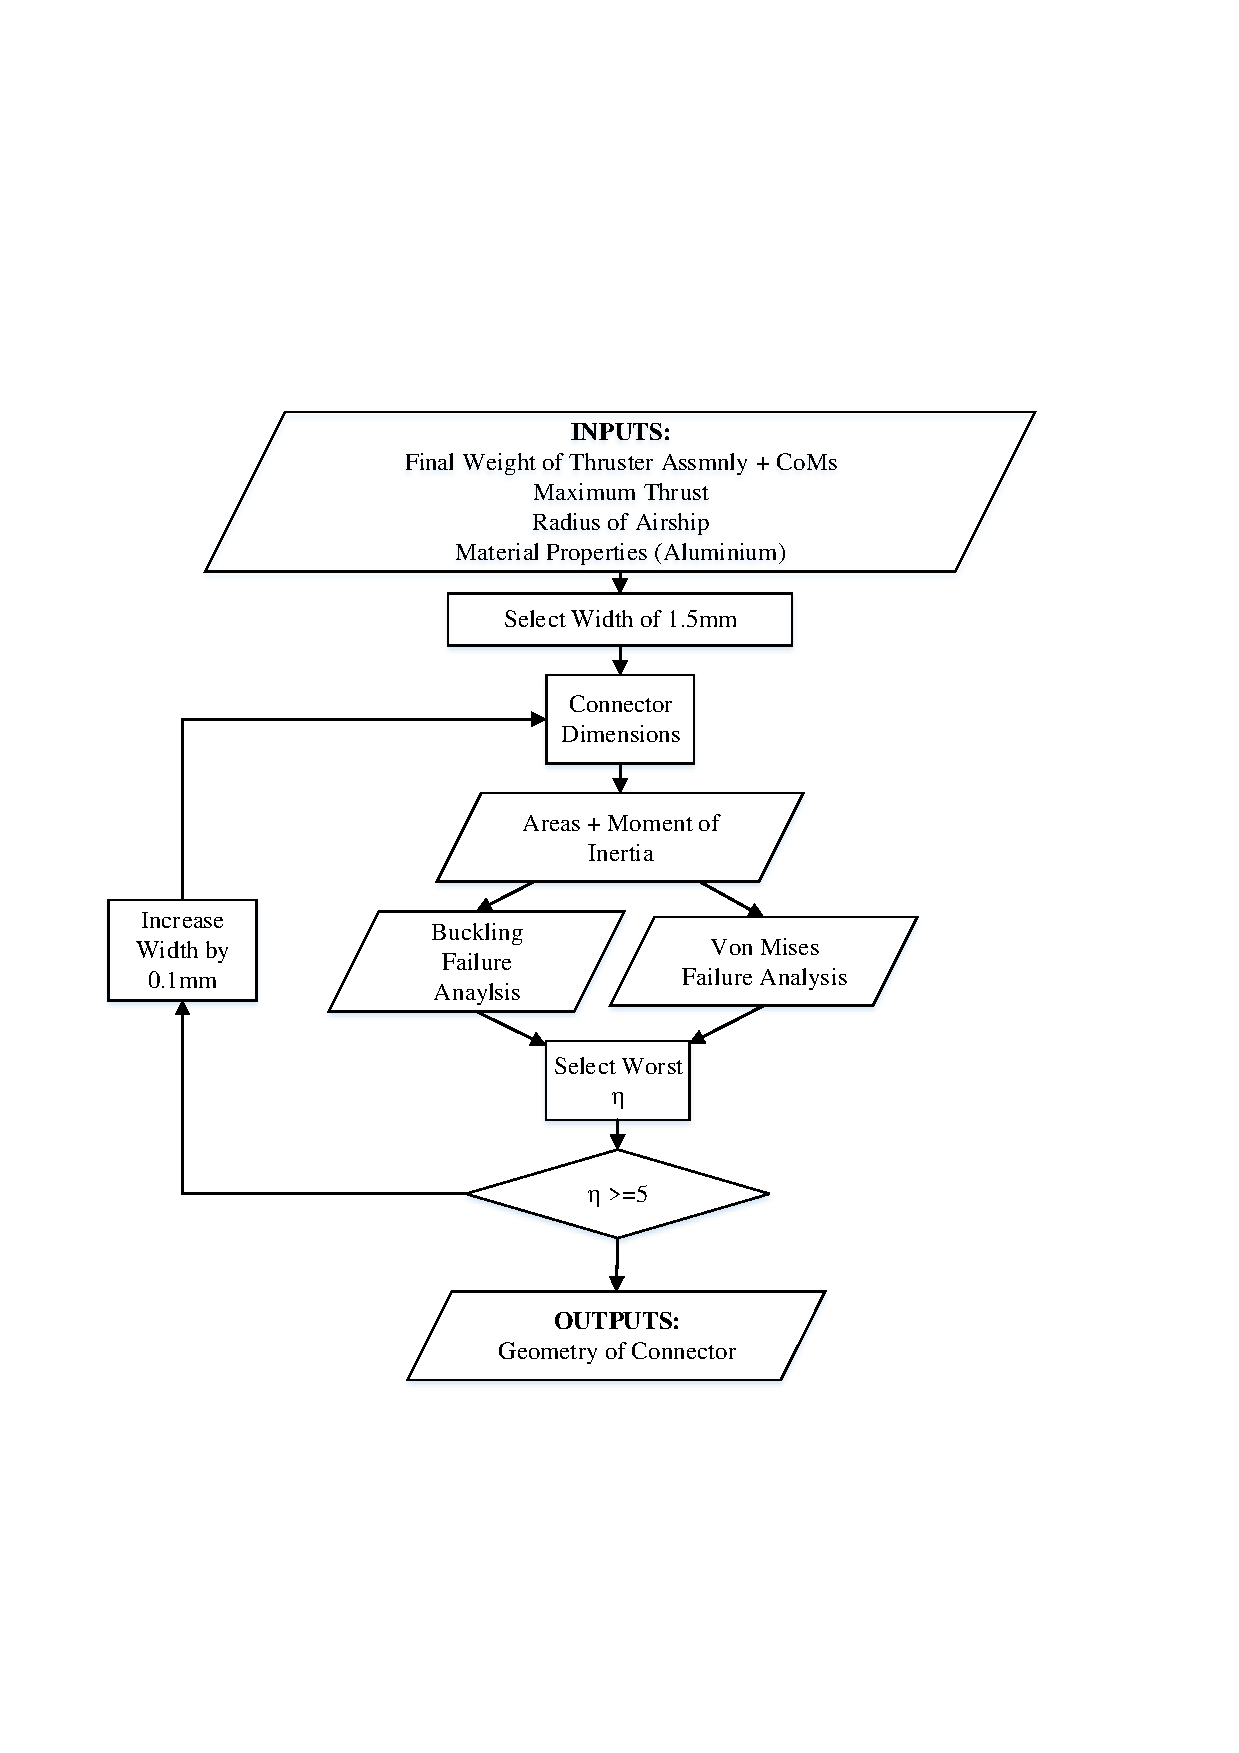
\includegraphics[width=.9\linewidth]{img/paramaterization/connector.pdf}
	\caption{Parametrization Outline for the Thruster Arm Connector}
	\label{fig:connectorParametrization}
\end{figure}

This section analyzes the thruster arms connection to the keel. It uses a rectangular piece that attaches into the bottom of the arm and the piece used for connecting the sections of keel together. The analysis output the geometry of the connector piece such that it meets the safety factor of 5 assigned to the component. The inputs required in order to preform the analysis incluide, the final weight of thruster assebmnly + CoMsMaximum ThrustRadius of AirshipMaterial Properties (Aluminium)

The first analysis relates to the loading scenario found in Figure \ref{fig:ArmThrustDown}. Where the connector holds the weight and thrusting forces in the z-direction. The inputs are the reaction forces from the arm. The assumption is that the two failures can occur from buckling and bending of the two pieces. A diagram of the top of the connector can be seen in Figure \ref{fig:KeelConnectionZ}, which calculates the reaction forces.\\

For the buckling failure, this could occur at the top part of the connector. Using the reaction forces found in Force Calculation section the cross section can be drawn, seen in Figure \ref{fig:ZDirCrossSect}


\noindent The buckling is calculated using Euler's critical load:

\begin{equation} \label{eqn:EulersCriticalForce}
P_{cr} = \frac{C\pi^2EI_z}{l^2}
\end{equation}
Where $C$ is an end constant taken as $1.2$ for this case, $E$ is the modulus of elasticity, $l$ is the height shown in Figure \ref{fig:ZDirCrossSect}, and $I_Z$ is calculated using:
\begin{equation}
I_z = \frac{b^3l}{12}
\end{equation}
Plugging these values into Equation \ref{eqn:EulersCriticalForce}:
\begin{equation}
P_{cr} = \frac{(1.2)\pi^2Eb^3}{12l}
\end{equation}
The safety factor is calculated using the force applied and the critical force (Equation \ref{eqn:EulersCriticalForce}):
\begin{equation}
\eta = \frac{P_{cr}}{F_{Rz}}
\end{equation}

\end{document}